% !TeX root = ../index.tex
\chapter{PHP \& Multimedia}
\graphicspath{{7-multimedia/images/}}

\section{Exercise 1}

\begin{figure}[H]
  \caption{Table created}
  \centering
  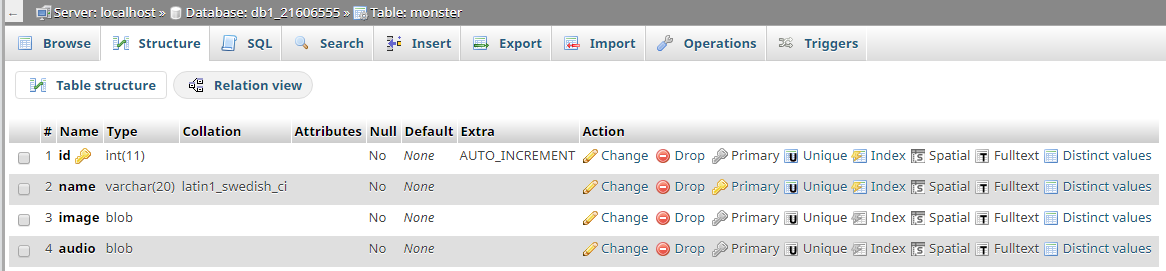
\includegraphics[width=\textwidth]{ex1}
\end{figure}

\clearpage
\section{Exercise 2}

\url{https://intweb.bucks.ac.uk/~21606555/oos/7-multimedia/ex2.html}

\captionsetup{type=figure}\captionof{figure}{ex2.html}
\subfile{pyg/src/7-multimedia/ex2}

\captionsetup{type=figure}\captionof{figure}{ex2-savemonster.php}
\subfile{pyg/src/7-multimedia/ex2-savemonster}

\begin{figure}[H]
  \caption{Upload form}
  \centering
  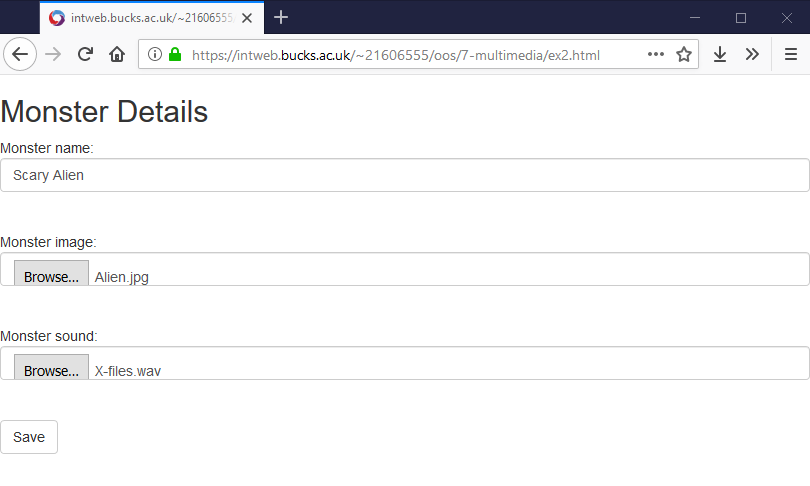
\includegraphics[width=\textwidth]{ex2-1upload}
\end{figure}

\begin{figure}[H]
  \caption{Uploaded data}
  \centering
  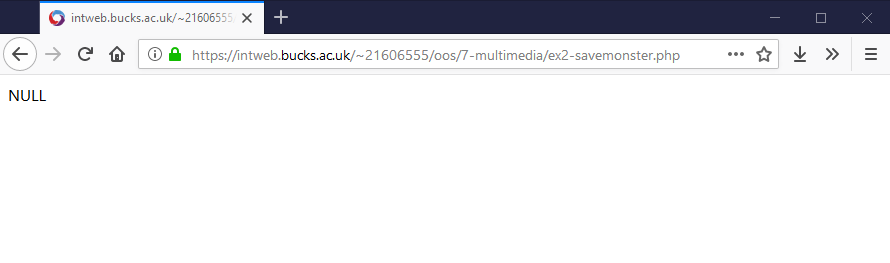
\includegraphics[width=\textwidth]{ex2-2uploaded}
\end{figure}

\begin{figure}[H]
  \caption{Data added to table}
  \centering
  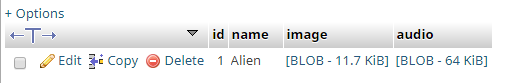
\includegraphics[width=\textwidth]{ex2-3result}
\end{figure}

\clearpage
\section{Exercise 3}

\url{https://intweb.bucks.ac.uk/~21606555/oos/7-multimedia/ex3-getjpg.php?id=1}\\\\
\url{https://intweb.bucks.ac.uk/~21606555/oos/7-multimedia/ex3-getwav.php?id=1}\\\\
\url{https://intweb.bucks.ac.uk/~21606555/oos/7-multimedia/ex3-displaymonster.php}

\captionsetup{type=figure}\captionof{figure}{ex3-getjpg.php}
\subfile{pyg/src/7-multimedia/ex3-getjpg}

\clearpage
\captionsetup{type=figure}\captionof{figure}{ex3-getwav.php}
\subfile{pyg/src/7-multimedia/ex3-getwav}

\captionsetup{type=figure}\captionof{figure}{ex3-displaymonster.php}
\subfile{pyg/src/7-multimedia/ex3-displaymonster}

\begin{figure}[H]
  \caption{Displaying image from database}
  \centering
  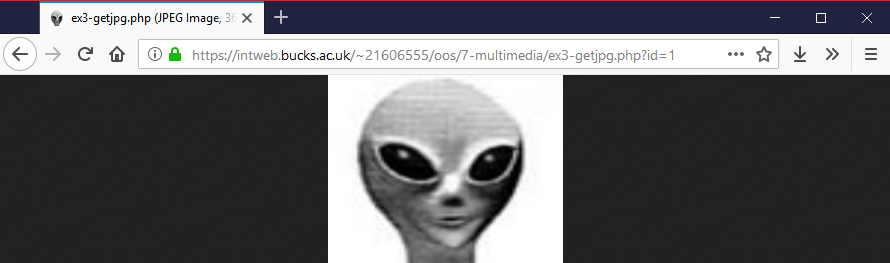
\includegraphics[width=\textwidth]{ex3-image}
\end{figure}

\begin{figure}[H]
  \caption{Displaying monster from database}
  \centering
  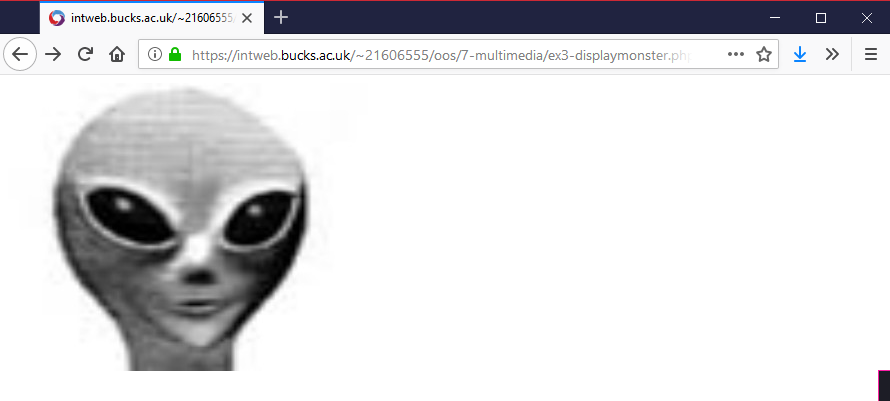
\includegraphics[width=\textwidth]{ex3-display}
\end{figure}

\clearpage
\section{Exercise 4}

\url{https://intweb.bucks.ac.uk/~21606555/oos/7-multimedia/ex4-displaymonster.php}

\captionsetup{type=figure}\captionof{figure}{ex4-displaymonster.php}
\subfile{pyg/src/7-multimedia/ex4-displaymonster}

\begin{figure}[H]
  \caption{Displaying all monsters in the database}
  \centering
  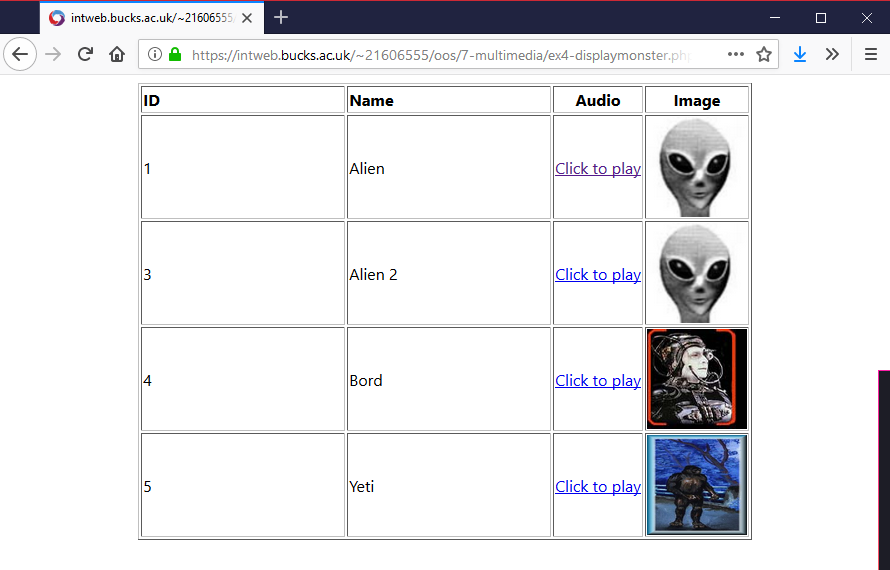
\includegraphics[width=\textwidth]{ex4}
\end{figure}

\clearpage
\section{Exercise 5}

\url{https://intweb.bucks.ac.uk/~21606555/oos/7-multimedia/ex5.php}

\captionsetup{type=figure}\captionof{figure}{ex5.php}
\subfile{pyg/src/7-multimedia/ex5}

\begin{figure}[H]
  \caption{Combining the image and audio scripts (image)}
  \centering
  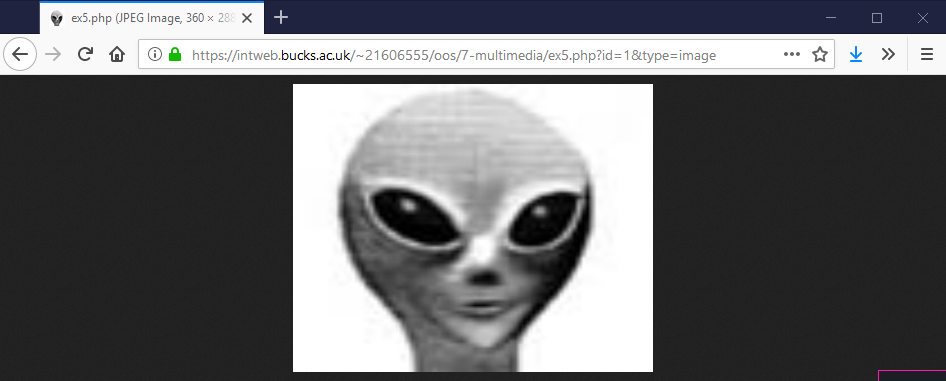
\includegraphics[width=\textwidth]{ex5-image}
\end{figure}

\begin{figure}[H]
  \caption{Combining the image and audio scripts (audio)}
  \centering
  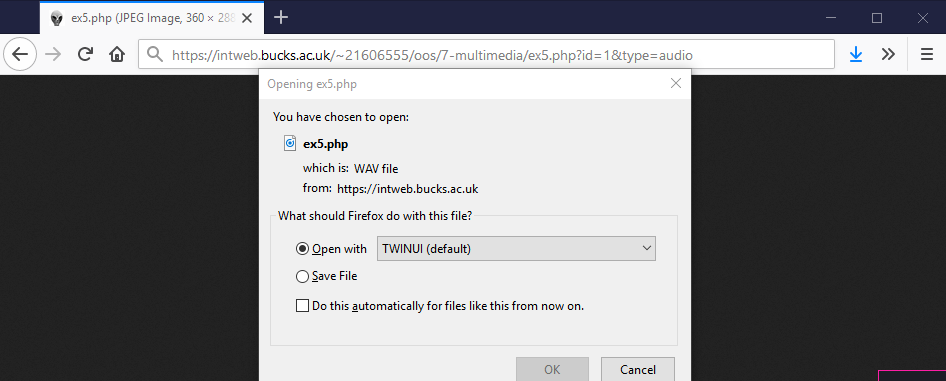
\includegraphics[width=\textwidth]{ex5-audio}
\end{figure}

\clearpage
\section{Exercise 6}

Sequence diagram of the script created in Exercise 5 being used.

\begin{figure}[H]
  \caption{UML Sequence Diagram}
  \centering
  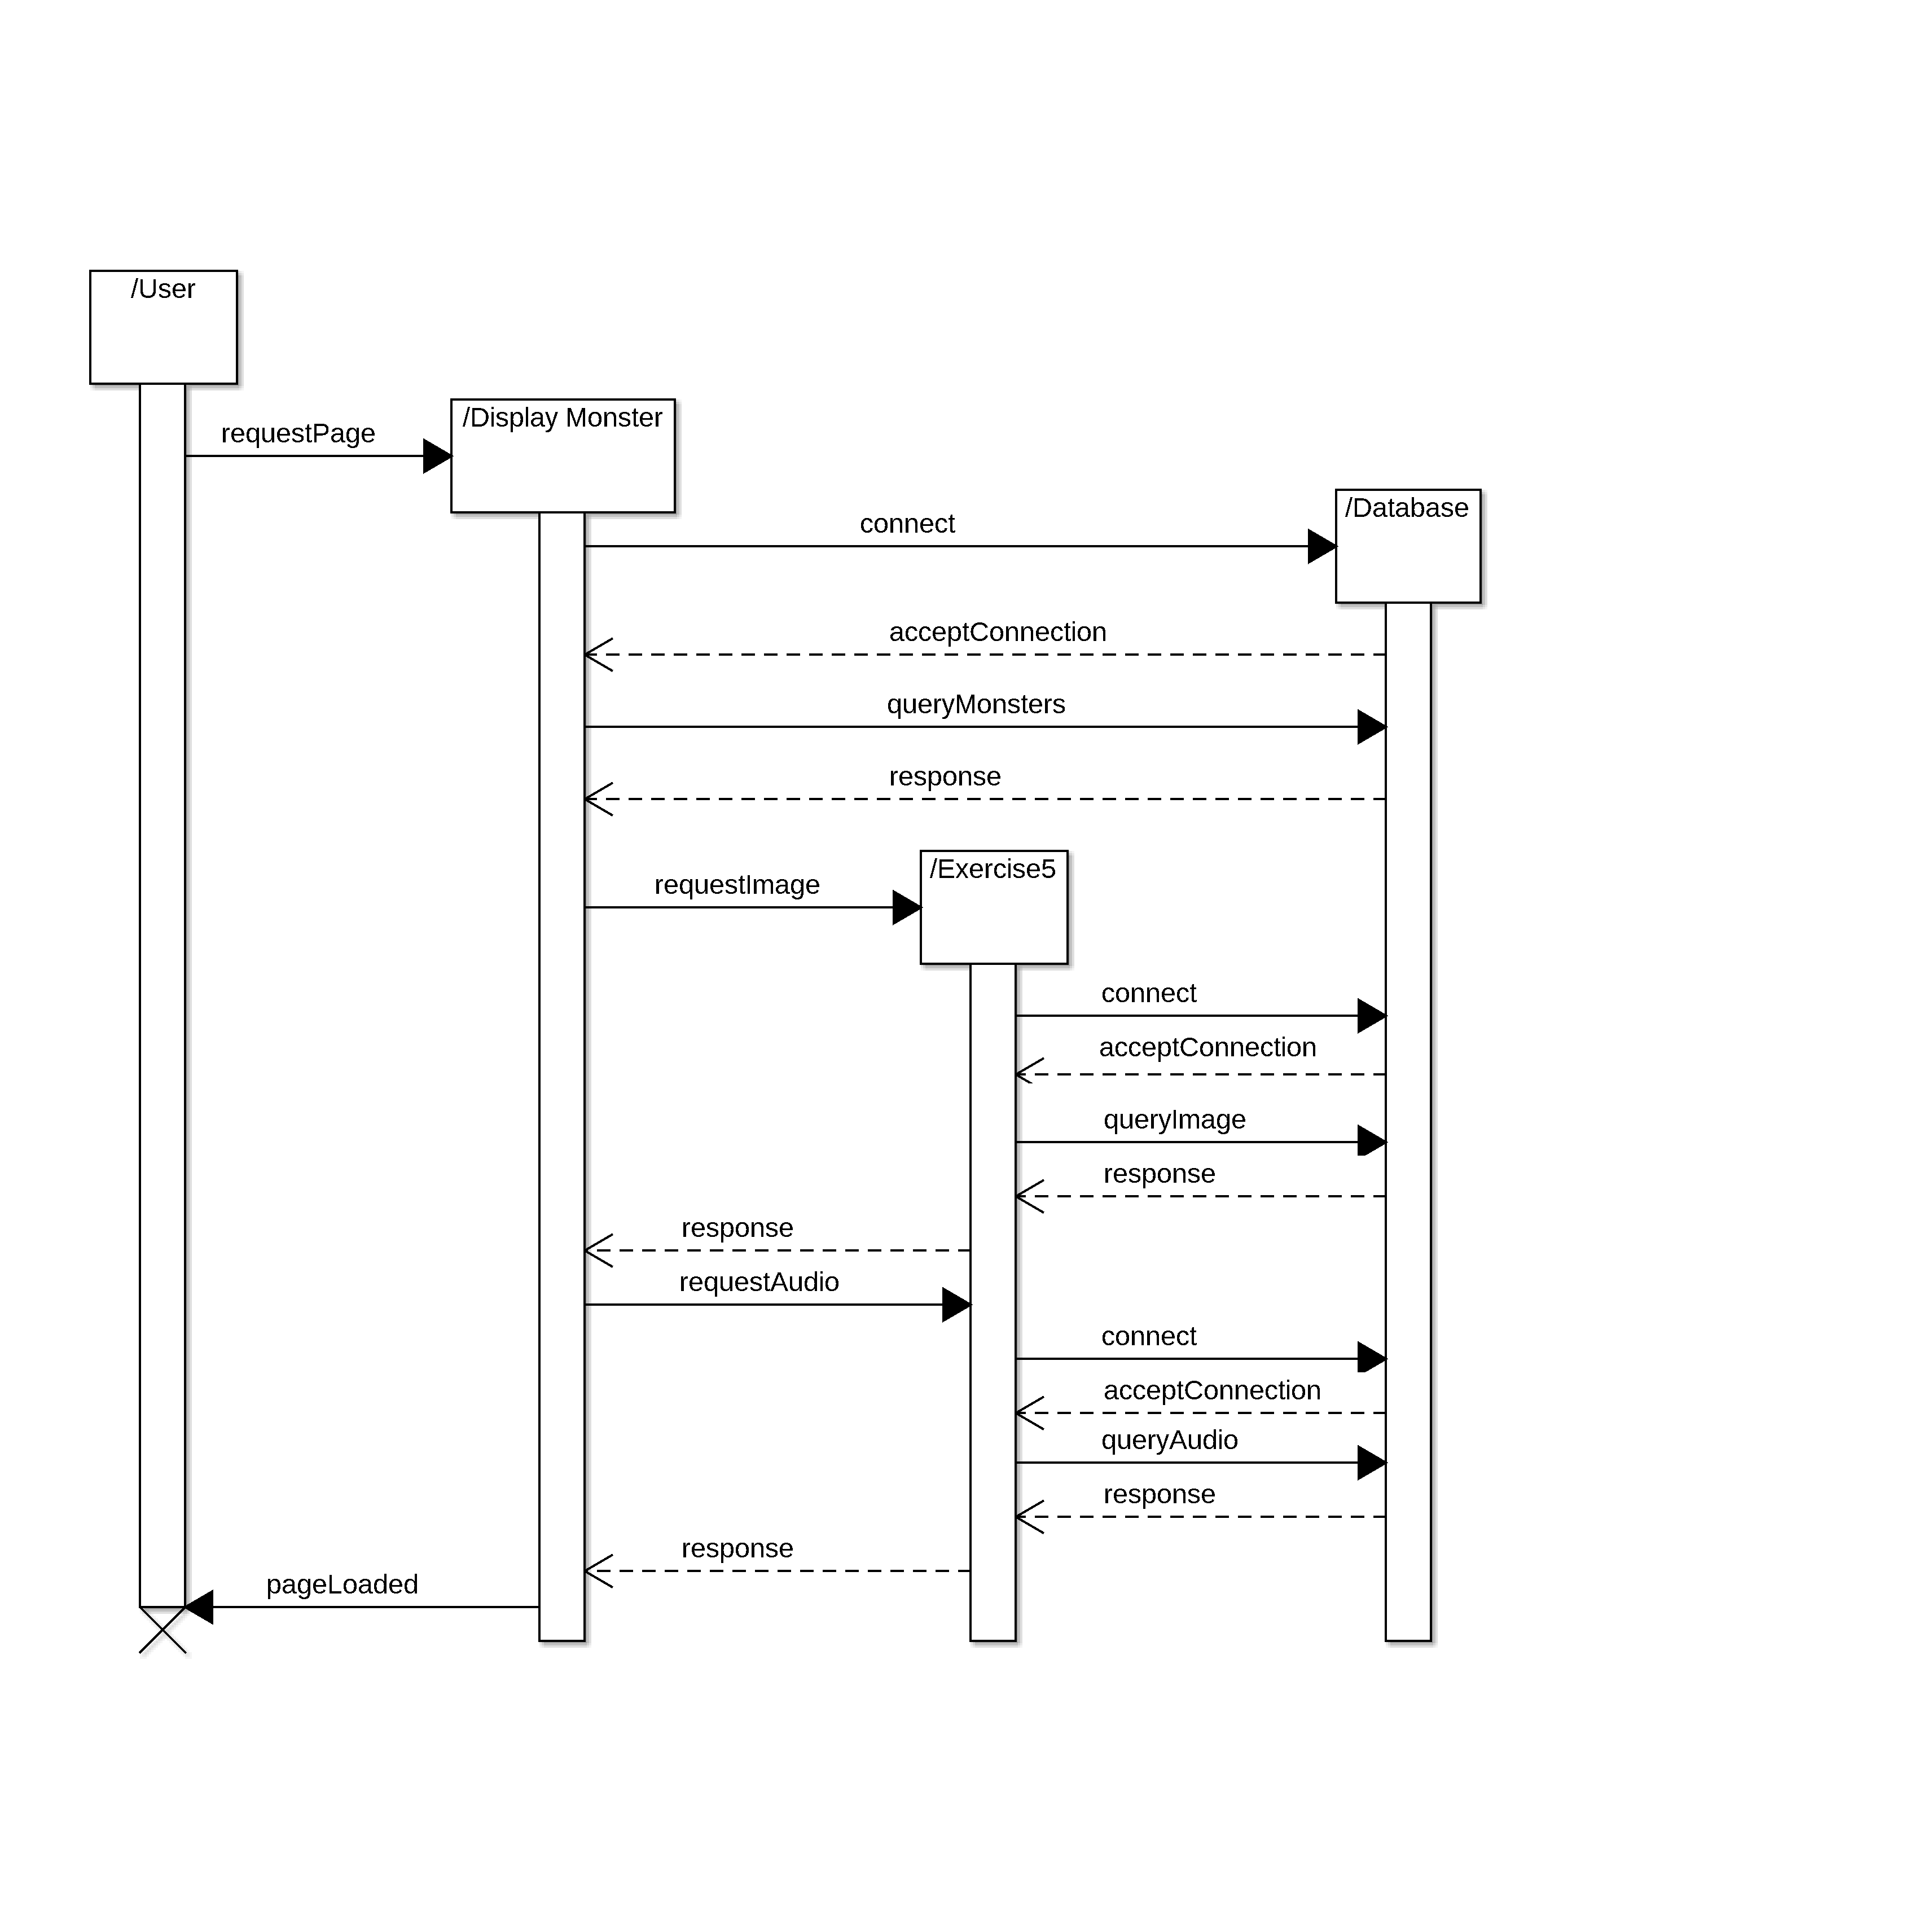
\includegraphics[width=1.25\textwidth]{sequence-diagram}
\end{figure}
